\documentclass[10pt]{article}
\usepackage[polish]{babel}
\usepackage[utf8]{inputenc}
\usepackage[T1]{fontenc}
\usepackage{amsmath}
\usepackage{amsfonts}
\usepackage{amssymb}
\usepackage[version=4]{mhchem}
\usepackage{stmaryrd}
\usepackage{graphicx}
\usepackage[export]{adjustbox}
\graphicspath{ {./images/} }

\title{LIGA MATEMATYCZNA im. Zdzisława Matuskiego GRUDZIEŃ 2016 SZKOŁA PODSTAWOWA }

\author{}
\date{}


\begin{document}
\maketitle
\section*{ZADANIE 1.}
Mikołaj napisał kolejne liczby naturalne używając łącznie siedmiu cyfr. Znajdź te liczby wiedząc, że ponad połowa spośród użytych cyfr była taka sama.

\section*{ZADANIE 2.}
Każdy uczestnik mikołajkowego turnieju dostaje dziesięć punktów na starcie i musi odpowiedzieć na 10 pytań. Za dobrą odpowiedź dostaje 1 punkt, za złą odpowiedź lub jej brak traci 1 punkt. Mikołaj ukończył turniej z 14 punktami. Ilu dobrych odpowiedzi udzielił?

\section*{ZADANIE 3.}
Mianownik pewnego ułamka jest o 3 większy od licznika. Jeżeli jego licznik zwiększymy o 10, a mianownik zwiększymy o 1 , to otrzymany ułamek będzie odwrotnością poszukiwanego. Jaki to ułamek?

\section*{ZADANIE 4.}
Ania rozpoczęła czytanie książki w sobotę. Przez pierwsze cztery dni czytała każdego dnia średnio po 12 stron. Przez następne dni czytała dziennie po 20 stron. Ostatniego dnia przeczytała ostatnie 10 stron książki. Okazało się, że gdyby czytała po 14 stron dziennie, to całą książkę przeczytałaby w tym samym czasie. Ile dni zajęło Ani przeczytanie tej książki? W którym dniu tygodnia skończyła czytać?

\section*{ZADANIE 5.}
Prostokąt przedstawiony na rysunku podzielono na sześć figur. Czworokąty \(A, B, C, D\) są kwadratami. Pole kwadratu \(A\) jest równe \(9 \mathrm{~cm}^{2}\), pole \(B-4 \mathrm{~cm}^{2}\), a pole \(D-49 \mathrm{~cm}^{2}\). Oblicz pole tego prostokąta.\\
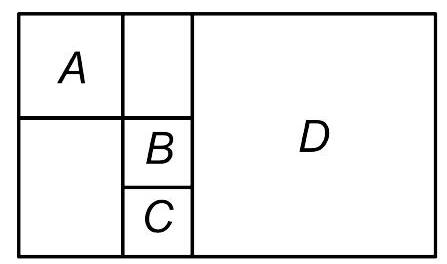
\includegraphics[max width=\textwidth, center]{2024_11_21_175fed1d19e2e2068a8dg-1}


\end{document}